\documentclass[11pt,a4paper]{article}

% ── Packages ──
\usepackage[utf8]{inputenc}
\usepackage[T1]{fontenc}
\usepackage{times}
\usepackage[margin=2cm]{geometry}
\usepackage{graphicx}
\usepackage{booktabs}
\usepackage{amsmath}
\usepackage{hyperref}
\usepackage{caption}
\usepackage{subcaption}
\usepackage{float}
\usepackage{enumitem}
\usepackage{xcolor}
\usepackage{listings}
\usepackage{array}
\usepackage{multirow}
\usepackage{fancyhdr}
\usepackage{tabularx}

\hypersetup{colorlinks=true,linkcolor=blue!60!black,citecolor=blue!60!black,urlcolor=blue!60!black}

\lstset{
  basicstyle=\ttfamily\scriptsize,
  keywordstyle=\color{blue!70!black}\bfseries,
  commentstyle=\color{green!50!black},
  stringstyle=\color{red!60!black},
  breaklines=true,
  frame=single,
  backgroundcolor=\color{gray!8},
  numbers=left,
  numberstyle=\tiny\color{gray},
  numbersep=5pt
}

\pagestyle{fancy}
\fancyhf{}
\fancyhead[L]{\small SupplyGraphOps}
\fancyhead[R]{\small Generative AI - Final Project}
\fancyfoot[C]{\thepage}
\renewcommand{\headrulewidth}{0.4pt}

% ── Title ──
\title{
  \textbf{SupplyGraphOps: Benchmark-Routed GraphRAG\\for Supply Chain Intelligence}\\[6pt]
  \large Generative AI - Final Project Report\\
  College of Computing
}

\author{
  Othmane AZOUBI \and Mohammed Rida ELHANI \and Yahya MANSOUB\\[6pt]
  \normalsize Supervised by: Pr.\ Lamiae AZIZI
}

\date{March 2026}

\begin{document}
\maketitle
\thispagestyle{fancy}

% ══════════════════════════════════════════════
\begin{abstract}
This report presents \textbf{SupplyGraphOps}, a supply-chain intelligence assistant that combines Graph-based Retrieval-Augmented Generation (GraphRAG) with large language model reasoning to support operational decision-making. We benchmark three retrieval strategies-Gemini Semantic RAG, GraphRAG (subgraph-as-context), and Text2Cypher (NL2Query)-over a structured supply chain knowledge graph derived from the SupplyGraph dataset. Core generation uses free-tier models (Gemma~3~27B for generation, \texttt{gemini-embedding-001} for embeddings), and evaluation is reported in two phases: an initial Gemma-as-judge baseline and an updated DeepSeek-judge benchmark to reduce same-model bias. Using LLM-as-judge evaluation, we show that each approach dominates on a distinct query class: Text2Cypher on exact lookups, GraphRAG on relational/semantic reasoning, and Semantic RAG on narrative synthesis. Based on these findings, we implement a deterministic intent-routing architecture deployed as the \textbf{EventualSmartFactory} dashboard-a production-style application combining visual analytics, risk monitoring, and an AI copilot. We discuss the business implications, supported by industry evidence showing that AI-driven supply chain intelligence can reduce operational costs by 15-24\% and cut manual interventions by up to 50\%.
\end{abstract}

% ══════════════════════════════════════════════
\section{Introduction}

Modern supply chains generate significant volumes of operational data-production counts, delivery metrics, sales orders, and factory issues-yet decision-makers often struggle to derive actionable intelligence from this fragmented information. The core challenge is not data scarcity but \textit{fragmented context}: product relationships and daily operational signals are spread across multiple files and systems, making rapid triage and confident decision-making difficult.

Recent advances in Retrieval-Augmented Generation (RAG) offer a promising path toward conversational supply chain analytics. By grounding large language model (LLM) responses in retrieved evidence, RAG systems can produce factual, traceable answers rather than hallucinated speculation. However, standard vector-based RAG treats documents as independent chunks, discarding the relational structure that is fundamental to supply chain data.

This project investigates \textbf{GraphRAG}-retrieval that exploits graph topology at query time-alongside two complementary approaches (Semantic RAG and Text2Cypher), applied to the SupplyGraph dataset. The project was developed as an experimental prototype using exclusively free-tier APIs (Google Gemma~3~27B and Gemini Embedding) to validate the viability of graph-based RAG for supply chain intelligence before committing to paid infrastructure.

Our contributions are fourfold. First, we provide a systematic benchmark of three retrieval strategies across four question types (structural, analytical, semantic, reasoning). Second, we demonstrate that no single approach dominates all query types, motivating a hybrid routing architecture. Third, we deliver \textbf{EventualSmartFactory}, a production-style dashboard implementing deterministic intent routing with an AI copilot. Fourth, we analyze business implications for supply chain operations teams, grounded in industry cost-savings evidence.

% ══════════════════════════════════════════════
\section{Related Work}

\subsection{Retrieval-Augmented Generation}

RAG was introduced by Lewis et al.\ to address hallucination in LLMs by grounding generation in retrieved external evidence. Standard RAG pipelines embed documents as vectors, retrieve top-$k$ chunks by cosine similarity, and pass them as context to an LLM. While effective for text corpora, this approach treats each chunk independently and cannot express relational dependencies between retrieved elements.

Recent improvements to RAG include multi-step retrieval, re-ranking, and iterative refinement, but these still operate over flat document collections. For domains where data is inherently relational-supply chains, knowledge graphs, biological networks-flat retrieval discards structural information that is often critical for answering complex queries.

\subsection{Graph-Based RAG and Microsoft GraphRAG}

GraphRAG extends retrieval to leverage graph structure. Rather than retrieving flat documents, it identifies seed entities in a knowledge graph and traverses edges to build a contextual subgraph. The term was formalized by Microsoft Research in their 2024 paper ``From Local to Global: A Graph RAG Approach to Query-Focused Summarization'' (Edge et al., 2024), which proposed a two-stage approach: first deriving an entity knowledge graph from source documents via LLM extraction, then pregenerating community summaries using the Leiden algorithm for hierarchical clustering. Given a query, community summaries generate partial responses that are aggregated into a final answer. Microsoft's results showed that GraphRAG substantially outperformed conventional vector RAG on global sensemaking questions over datasets in the million-token range, for both comprehensiveness and diversity of generated answers.

Several open-source implementations have emerged in this space, including Microsoft's own GraphRAG library, Nano-GraphRAG, Fast GraphRAG, and LightRAG, as well as domain-specific adaptations for geosciences and mining. Our work differs from Microsoft's approach in that we apply GraphRAG to a \textit{structured} supply chain knowledge graph with explicit node types and relationships, rather than extracting entities from unstructured text. Our subgraph-as-context retrieval traverses the existing graph topology at query time, while Microsoft's approach builds the graph from scratch during indexing.

\subsection{NL2Query Approaches}

Text2Cypher (and Text2SQL) methods bypass embedding-based retrieval entirely by having an LLM generate a database query from natural language. These approaches offer exact precision on structured queries-a Cypher \texttt{SUM} will always be correct if the query is valid. However, they are fragile when questions require open-ended reasoning, when the LLM generates syntactically invalid queries, or when the question does not map cleanly to a single query pattern.

The trade-off is between precision and coverage: NL2Query gives exact answers to narrow questions, while RAG gives approximate answers to broad questions. This complementarity motivates hybrid architectures.

\subsection{Supply Chain AI}

The SupplyGraph dataset (Aziz et al., 2024) provides a benchmark for graph-based supply chain analytics, modeling products as nodes with temporal observation series and structural relationships through plants, storage locations, and product groupings. Prior work on SupplyGraph has focused on GNN-based forecasting tasks such as demand prediction and anomaly detection. Our work is the first to apply RAG-based conversational intelligence to this dataset, treating it as a knowledge base for operational question-answering rather than a prediction benchmark.

\subsection{LLM-as-Judge Evaluation}

Evaluating open-ended question-answering systems is inherently difficult. Traditional metrics like BLEU, ROUGE, or Precision@$K$ fail to capture answer quality for reasoning or synthesis tasks. The LLM-as-judge paradigm, where a capable LLM scores answers on criteria such as correctness, completeness, and clarity, has emerged as a practical alternative. Microsoft's GraphRAG paper itself used this approach for evaluation. While not without bias (the judge may favor verbose or well-formatted answers regardless of accuracy), it scales better than human evaluation and captures dimensions that automated metrics miss.

% ══════════════════════════════════════════════
\section{Dataset and Knowledge Graph}

\subsection{SupplyGraph Dataset}

The SupplyGraph dataset models a supply chain with \textbf{40~products} represented as nodes. Each product has attributes including product code, group, and subgroup. Edges encode structural relationships: products are assigned to plants, stored in storage locations, and grouped by product family.

Temporal data is recorded as daily observations per product across four metrics: \textit{delivery}, \textit{production}, \textit{sales\_order}, and \textit{factory\_issue}, each measured in both unit and weight dimensions.

\subsection{Neo4j Knowledge Graph}

We construct a knowledge graph in Neo4j with the following schema. \textbf{Product} nodes (40) carry attributes for code, group, and subgroup. \textbf{Plant} nodes represent factory identifiers, and \textbf{Storage} nodes represent storage location identifiers. \textbf{Observation} nodes (approximately 70{,}700) record daily metric values. Relationships include \texttt{ASSIGNED\_TO\_PLANT}, \texttt{STORED\_IN}, and \texttt{HAS\_OBSERVATION}. The full graph contains \textbf{70{,}798~nodes} and \textbf{71{,}272~edges}.

A key modeling constraint is that temporal data is aggregated by product and date, not split by plant. Plant and storage are therefore treated as structural dependency context rather than direct temporal dimensions.

\begin{figure}[H]
\centering
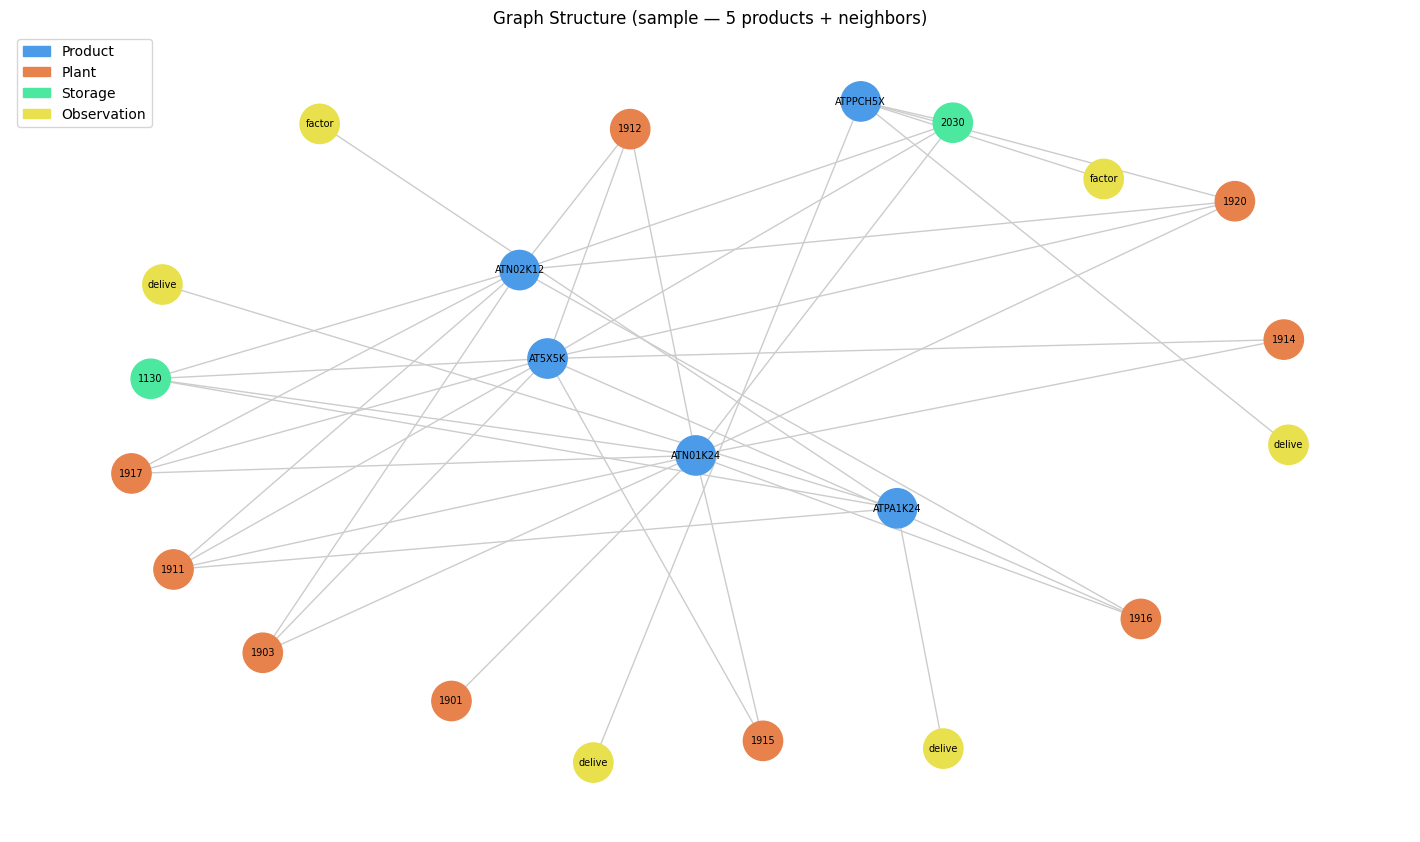
\includegraphics[width=0.95\linewidth]{figures/neo4j_graph.png}
\caption{Neo4j graph visualization showing product nodes, plant and storage connections, and observation leaves. The graph contains 70{,}798 nodes and 71{,}272 edges.}
\label{fig:neo4j}
\end{figure}

% ══════════════════════════════════════════════
\section{Data Exploration and Preprocessing}

Before building the RAG pipeline, a systematic exploratory data analysis (EDA) was conducted to understand the dataset structure, assess data quality, and produce the cleaned tables needed for Neo4j ingestion. This phase was critical for identifying modeling constraints that shaped the subsequent retrieval architecture.

\subsection{File Inventory and Data Loading}

The SupplyGraph repository organizes raw data into three families. Node files contain a single master table of 40 product codes with group and subgroup attributes. Edge files encode structural relationships (product-to-plant, product-to-storage, product-group, product-subgroup) in both label and index formats. Temporal data files provide daily observations in wide format, with one CSV per metric (delivery, production, sales\_order, factory\_issue) and per unit type (unit, weight), totaling 8 temporal files.

All CSVs were loaded and inventoried programmatically. The temporal files contained between 365 and 730 rows (one per date) and 41 columns (Date + 40 product columns), confirming the dataset spans approximately 1-2 years of daily observations.

\subsection{Data Quality Assessment}

A generic quality audit was applied across all loaded DataFrames, computing row counts, duplicate rows, missing values per column, and type consistency. Several issues were identified and resolved.

In the temporal files, some product codes appeared with a \texttt{.1} suffix due to pandas column deduplication when duplicate column headers existed in the raw CSVs. A canonicalization step stripped these suffixes and summed the values of merged columns. Date columns were parsed and validated, confirming no missing or malformed dates. Numeric columns were checked for negative values (none found) and zero-rate sparsity was computed per file. Some metrics exhibited high sparsity (over 60\% zeros for factory\_issue), which is expected-most products do not experience factory issues on most days.

In the edge files, duplicate pairs were found to encode edge strength (the number of times two products co-occur in the same context). Both weighted (preserving duplicates as edge weight) and unweighted (deduplicated) graph views were constructed.

\subsection{Temporal Reshaping}

The raw temporal data was in wide format (products as columns), which is unsuitable for graph-based analysis. A reshaping pipeline melted each temporal file from wide to long format, producing a unified table \texttt{ts\_long} with schema: \texttt{date}, \texttt{node}, \texttt{metric}, \texttt{unit\_type}, \texttt{value}. This canonical representation enabled downstream pivoting for business diagnostics and was exported as \texttt{observations.csv} for Neo4j ingestion.

\subsection{Business-Focused Diagnostics}

Using the long-format temporal data, three diagnostic features were computed at the daily product level. \textbf{Demand gap} (\texttt{sales\_order $-$ delivery}) identifies products where customer demand exceeds fulfilled deliveries. \textbf{Supply gap} (\texttt{production $-$ sales\_order}) reveals production-demand mismatches. \textbf{Issue pressure} (\texttt{factory\_issue / production}) quantifies the proportion of production affected by factory issues, with division-by-zero handled by defaulting to zero.

Products with the largest average positive demand gap were flagged as candidates for supply chain risk analysis. Time series plots of selected products confirmed patterns of intermittent delivery shortfalls correlated with spikes in factory issues, validating the diagnostic features as meaningful operational signals.

\begin{figure}[H]
\centering
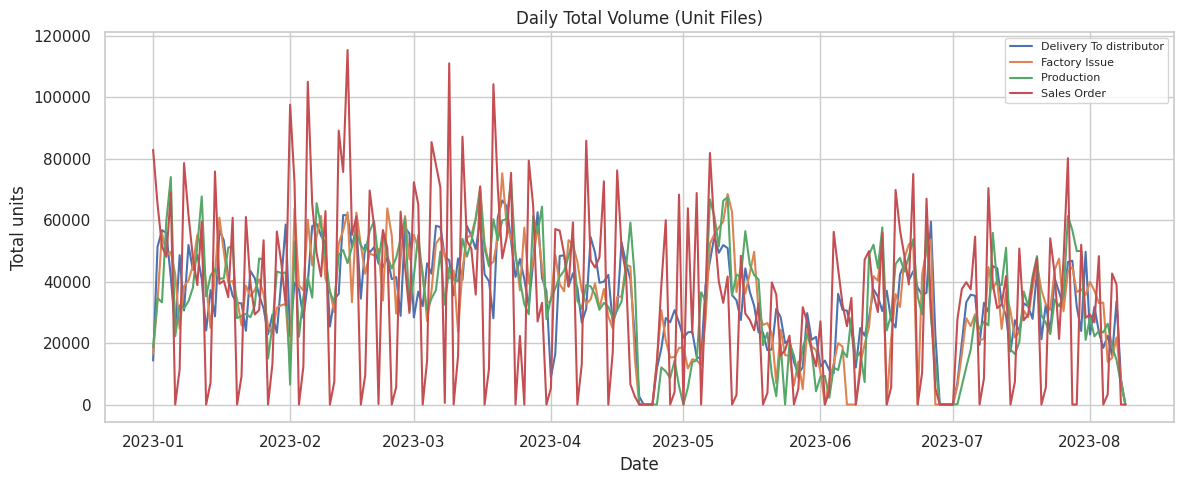
\includegraphics[width=0.95\linewidth]{figures/eda_daily_totals.png}
\caption{Daily total volume across all 40 products for each Unit metric (delivery, production, sales\_order, factory\_issue). The chart reveals seasonal patterns, demand-delivery gaps, and the relative sparsity of factory issue events.}
\label{fig:eda}
\end{figure}

\subsection{Graph-Temporal Linkage}

To assess whether graph topology correlates with temporal behavior, node degree (from the weighted edge graph) was merged with temporal volatility (coefficient of variation of daily values per product). This preliminary analysis generated hypotheses that informed the RAG architecture design: products with higher connectivity (more shared plants and storage locations) tended to show more stable delivery patterns, suggesting that structural context is informative for operational reasoning-a finding that supports the GraphRAG approach over flat document retrieval.

\subsection{Processed Output}

The EDA pipeline produced four cleaned, Neo4j-ready CSV files exported to a \texttt{Processed/} directory: \texttt{products.csv} (40 products with group and subgroup), \texttt{product\_plant.csv} (product-to-plant assignments), \texttt{product\_storage.csv} (product-to-storage assignments), and \texttt{observations.csv} (the full long-format temporal dataset). These files are automatically loaded by the EventualSmartFactory application's bootstrap service on first startup.

% ══════════════════════════════════════════════
\section{Methodology}

\subsection{Model Selection: Free-Tier Experimental Strategy}

A deliberate design decision was to use free-tier models for the core retrieval architecture. All text generation (RAG answers, Cypher generation, answer synthesis) uses \textbf{Gemma~3~27B} (\texttt{gemma-3-27b-it}) via Google AI Studio API. Embeddings use \textbf{gemini-embedding-001} with 256 dimensions. API calls are rate-limited with a 5-second sleep between requests to stay under the free tier limit of 15~RPM. For evaluation, we report both the original Gemma-as-judge run and an updated benchmark where \textbf{DeepSeek} is used as an independent judge.

This choice was intentional: before investing in paid API access (GPT-4o, Claude, or Gemini Pro), we wanted to establish whether the retrieval architecture itself-not the LLM quality-was the primary driver of answer quality. The results confirm that even with a mid-tier model, the routing architecture produces strong differentiation between approaches, validating the concept before scaling to production-grade LLMs.

Embeddings are cached to disk (\texttt{embeddings/gemini\_products.npz}) after first generation to avoid re-consuming API quota on repeated runs, a practical optimization for iterative development under rate-limited conditions.

\subsection{Discarded Approach: Node2Vec}

Node2Vec was initially considered as a structural embedding method. Training was launched on the full 70{,}798-node graph with parameters \texttt{num\_walks=200}, \texttt{walk\_length=30}, and ran for over 5~hours without completing.

The root cause was that approximately 70{,}700 Observation nodes are leaf nodes (degree~1), inflating the random walk space by roughly 1{,}700$\times$ with zero inter-product structural signal. Beyond this performance issue, Node2Vec was architecturally unsuitable for three reasons. First, it ignores node attribute values entirely-the actual supply chain metrics (delivery volumes, production rates, demand gaps) that carry operational significance are invisible to graph-walk embeddings. Second, queries must be embedded by a text model (Gemini), creating an \textbf{asymmetric retrieval space} where cosine similarity between text embeddings and graph-walk embeddings has no theoretical grounding. Third, with only 40 products and 64 embedding dimensions, the embedding space is massively underconstrained.

Node2Vec would be meaningful in a supply chain context with thousands of products, rich multi-hop dependency paths (product $\rightarrow$ component $\rightarrow$ supplier $\rightarrow$ plant), and purely topology-driven similarity tasks-conditions not met by this dataset. It was removed from the benchmark.

\subsection{Approach A: Gemini Semantic RAG}

For each of the 40 products, a rich text description is built from the graph by aggregating plant assignments, storage locations, and metric statistics (averages and totals for delivery, production, sales\_order, and factory\_issue in both unit and weight dimensions). Each description is then embedded with \texttt{gemini-embedding-001} using 256 dimensions and the \texttt{RETRIEVAL\_DOCUMENT} task type.

At query time, the question is embedded with the same model using the \texttt{RETRIEVAL\_QUERY} task type, and the top-$K$ products are retrieved by cosine similarity. The retrieved product descriptions are passed as context to Gemma~3~27B, which generates the final answer.

The key property of this approach is that query and documents share the same embedding space, making cosine similarity semantically meaningful. This contrasts with the Node2Vec approach where the embedding spaces are fundamentally incompatible.

\begin{figure}[H]
\centering
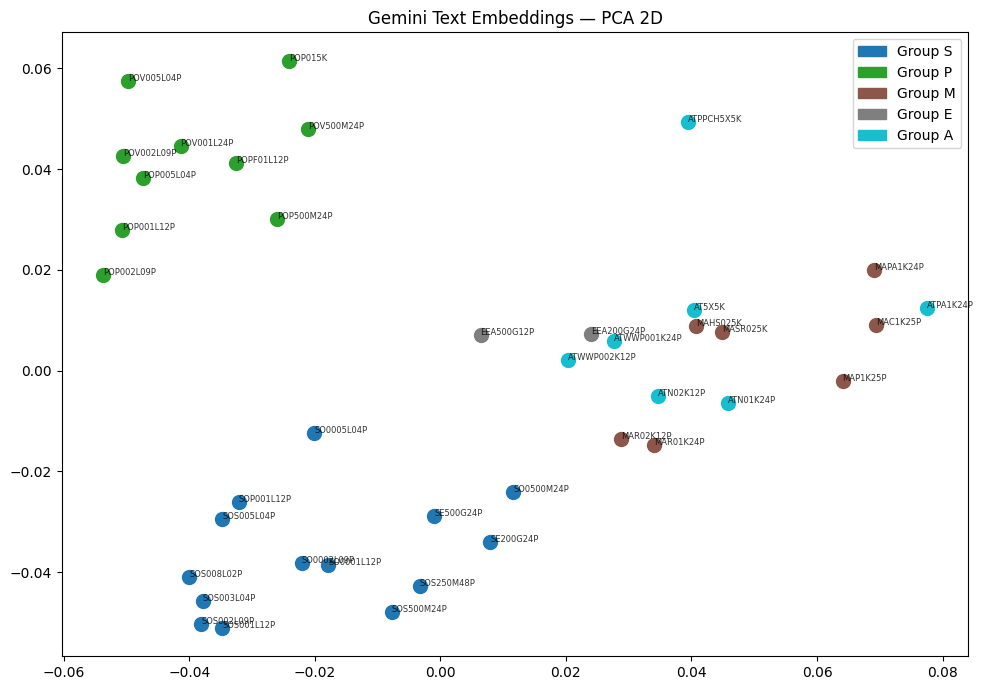
\includegraphics[width=0.8\linewidth]{figures/pca_embeddings.png}
\caption{PCA projection of Gemini product embeddings (256d $\rightarrow$ 2d), colored by product group. Same-group products cluster slightly closer (group ratio = 1.027), confirming modest behavioral similarity captured by the embedding model.}
\label{fig:pca}
\end{figure}

\subsection{Approach B: GraphRAG (Subgraph-as-Context)}

This is \textbf{genuine GraphRAG} in the sense that graph topology is used at retrieval time, not just at index time. The pipeline begins by embedding the query with \texttt{gemini-embedding-001} and finding the top matching product (seed node) by cosine similarity. From the seed node, the system \textbf{traverses the graph} in Neo4j to collect direct connections (assigned plants and storage locations), 2-hop neighbors (products sharing the same plants, which we call structural siblings, fetched via a second Cypher query), and aggregated metrics for both the seed product and its siblings.

The resulting subgraph-nodes, relationships, and attributes-is serialized as structured context and passed to Gemma~3~27B, which is explicitly prompted to reason over graph relationships.

The key distinction from Semantic RAG is that Semantic RAG retrieves $K$ independent product text documents, while GraphRAG retrieves 1~seed then expands through graph structure. The context therefore encodes \textit{who is connected to whom and via which shared infrastructure}, enabling the LLM to perform relational reasoning that flat document context cannot support. No additional API calls are required for graph traversal since all expansion is handled by Neo4j Cypher queries locally.

Our approach differs from Microsoft's GraphRAG in an important way: Microsoft's framework builds a knowledge graph from unstructured text via LLM extraction and uses community detection for hierarchical summarization. Our approach operates on an \textit{existing} structured graph with explicit typed relationships, and uses vector search only for seed selection before expanding through the known topology. This makes our method more suitable for domains where the graph structure is already defined by the data schema.

\subsection{Approach C: Text2Cypher (NL2Query)}

This approach is \textbf{not RAG}-it is a natural-language-to-query translation method. The graph schema (node types, relationships, available metrics) is provided as a prompt prefix to Gemma~3~27B, which generates a Cypher query from the natural language question. The generated query is executed directly on Neo4j, and the results are passed back to Gemma~3~27B for human-readable synthesis.

The key property is that there are no embeddings involved. The system accesses the graph directly, and results are exact rather than approximated. However, the approach is inherently fragile on open-ended questions where valid Cypher is difficult to generate, and it depends entirely on the LLM's ability to produce syntactically correct queries for the given schema.

% ══════════════════════════════════════════════
\section{Evaluation}

\subsection{LLM-as-Judge Protocol}

An initial evaluation using Precision@$K$ with manually set relevant codes was discarded as flawed. The ground truth was incomplete (for example, plant 1903 has 8 products but only 1 was marked relevant in the manual set), and binary metrics fundamentally cannot evaluate open-ended reasoning answers.

We adopt \textbf{LLM-as-judge} evaluation with three criteria (1-5 scale): \textbf{Correctness}, \textbf{Completeness}, and \textbf{Clarity}. The benchmark is reported in two phases:
\begin{itemize}[nosep]
  \item \textbf{Phase A (historical baseline):} Gemma~3~27B used as both generator and judge.
  \item \textbf{Phase B (current reference):} DeepSeek used as judge while generation remains Gemma~3~27B.
\end{itemize}
This separation reduces same-model bias in scoring while keeping the retrieval/generation architecture unchanged.

\subsection{Benchmark Questions}

The updated benchmark uses \textbf{20 questions} across four types to reduce variance and better represent enterprise question diversity:

\begin{table}[H]
\centering
\caption{Benchmark questions by type}
\label{tab:questions}
\scriptsize
\begin{tabularx}{\linewidth}{>{\raggedright\arraybackslash}p{2.2cm} >{\centering\arraybackslash}p{1.8cm} >{\raggedright\arraybackslash}X}
\toprule
\textbf{Type} & \textbf{Count} & \textbf{Examples} \\
\midrule
Structural & 5 & Product-plant assignments, group/subgroup membership, storage lookups \\
Analytical & 5 & Totals, top-$k$, and aggregate metrics by group/subgroup/plant \\
Semantic & 5 & Similar-product queries based on operational behavior \\
Reasoning & 5 & Bottlenecks, risk diagnosis, and corrective-action prioritization \\
\bottomrule
\end{tabularx}
\end{table}

% ══════════════════════════════════════════════
\section{Results}

\subsection{Overall Scores}

\begin{table}[H]
\centering
\caption{Overall benchmark scores (20 questions, DeepSeek judge, avg 1-5)}
\label{tab:overall}
\begin{tabular}{lcc}
\toprule
\textbf{Approach} & \textbf{Avg Score} & \textbf{Type} \\
\midrule
GraphRAG & \textbf{4.20} & Graph-traversal RAG \\
Gemini Semantic RAG & 4.17 & Semantic RAG \\
Text2Cypher & 3.62 & NL2Query \\
\bottomrule
\end{tabular}
\end{table}

\subsection{Per-Type Analysis}

\begin{table}[H]
\centering
\caption{Average score by question type (20-question DeepSeek run)}
\label{tab:pertype}
\scriptsize
\begin{tabularx}{\linewidth}{>{\raggedright\arraybackslash}p{2.2cm} >{\centering\arraybackslash}p{1.7cm} >{\centering\arraybackslash}p{1.7cm} >{\centering\arraybackslash}p{1.7cm} >{\raggedright\arraybackslash}X}
\toprule
\textbf{Question Type} & \textbf{Gemini} & \textbf{T2C} & \textbf{GraphRAG} & \textbf{Winner Pattern} \\
\midrule
Structural & 5.00 & 5.00 & 4.73 & Gemini/Text2Cypher tie \\
Analytical & 3.67 & \textbf{4.20} & 3.27 & Text2Cypher \\
Semantic & 3.60 & 2.20 & \textbf{4.33} & GraphRAG \\
Reasoning & 4.40 & 3.07 & \textbf{4.47} & GraphRAG \\
\bottomrule
\end{tabularx}
\end{table}

\subsection{Embedding Quality}

Gemini embeddings show modest but positive group coherence:

\begin{table}[H]
\centering
\caption{Embedding similarity analysis}
\label{tab:embedding}
\begin{tabular}{lc}
\toprule
\textbf{Metric} & \textbf{Value} \\
\midrule
Intra-group avg cosine sim. & 0.9517 \\
Inter-group avg cosine sim. & 0.9266 \\
Group ratio (intra/inter) & \textbf{1.027} \\
\bottomrule
\end{tabular}
\end{table}

A group ratio above 1.0 confirms that same-group products cluster together in embedding space, though the effect is modest given the 40-product corpus. This suggests that the Gemini embedding model captures some behavioral similarity from the aggregated metric descriptions, but the limited number of products constrains the separation achievable.

\subsection{Observations}

\textbf{Text2Cypher remains best for exact graph analytics.} In the 20-question run, it leads analytical questions (4.20) and ties for structural questions (5.00), confirming that NL2Query is the strongest option for strict lookups, counts, and aggregations.

\textbf{GraphRAG is strongest on semantic and reasoning intents.} It leads semantic (4.33) and reasoning (4.47) categories, and has the highest overall average (4.20), indicating better performance when answers require relational context and multi-entity interpretation.

\textbf{Gemini RAG remains a strong narrative fallback.} Despite a slightly lower overall average (4.17), it stays competitive and is valuable when users ask broad narrative synthesis questions that do not require strict database precision.

\textbf{Bias handling improvement.} The earlier Gemma-as-judge baseline raised a leniency concern (well-written partial answers being overrated). The DeepSeek-judge rerun keeps generation fixed while changing the evaluator, reducing same-model bias and increasing confidence in architecture-level conclusions.

\begin{figure}[H]
\centering
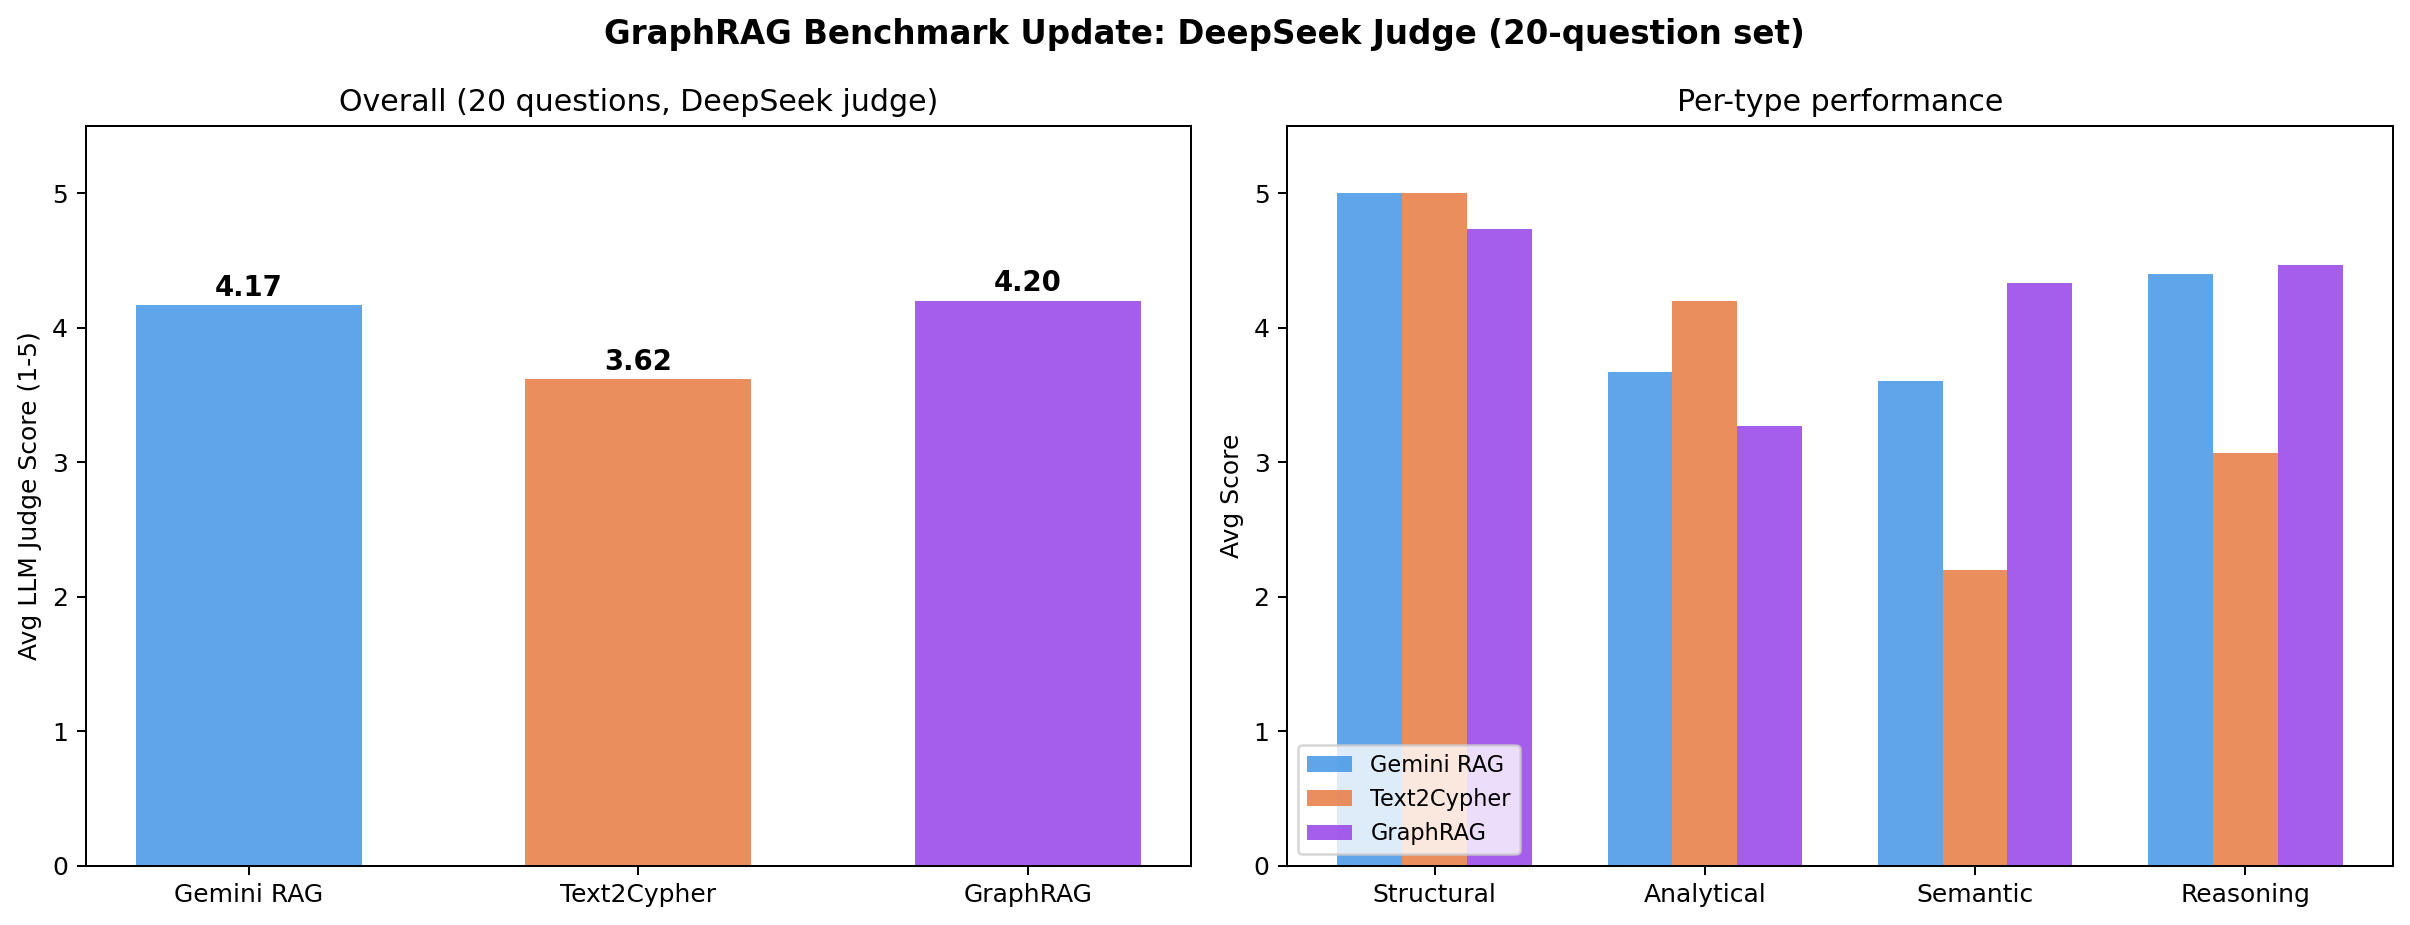
\includegraphics[width=0.95\linewidth]{figures/benchmark_bars.png}
\caption{Benchmark plots from the 20-question DeepSeek-judge run: overall averages and per-type performance for Gemini RAG, Text2Cypher, and GraphRAG.}
\label{fig:benchmark}
\end{figure}

% ══════════════════════════════════════════════
\section{Intent-Routing Architecture}

Based on benchmark findings, we implement a \textbf{deterministic intent router} that dispatches queries to the optimal strategy.

\subsection{Routing Logic}

The router (\texttt{IntentRouterService}) operates as a sequential classifier. First, it performs \textbf{structured-intent detection}: if the question contains analytical keywords (\texttt{how many}, \texttt{count}, \texttt{total}, \texttt{sum}, \texttt{average}, \texttt{list}) combined with schema-oriented entities (\texttt{plant}, \texttt{group}, \texttt{subgroup}, \texttt{storage}), the query is routed to \textbf{Text2Cypher}. If the question does not match the structured pattern, the router checks for \textbf{relational/reasoning intent} using keywords such as \texttt{similar}, \texttt{related}, \texttt{compare}, \texttt{risk}, \texttt{bottleneck}, \texttt{anomaly}, or reasoning cues like \texttt{why} and \texttt{how...affect}-these are routed to \textbf{GraphRAG}. All remaining queries default to \textbf{Semantic RAG} for open-ended narrative synthesis.

\subsection{Fallback Mechanism}

If Text2Cypher fails to produce a safe read-only Cypher query or if query execution fails, the system automatically falls back to GraphRAG. Safety checks block write and destructive operations including \texttt{CREATE}, \texttt{MERGE}, \texttt{DELETE}, \texttt{SET}, \texttt{CALL}, and \texttt{APOC} procedures. This ensures that the copilot never modifies the graph and that users always receive a response even when Cypher generation fails.

\subsection{Benchmark Alignment}

\begin{table}[H]
\centering
\caption{Routing policy derived from benchmark results}
\label{tab:routing}
\scriptsize
\begin{tabularx}{\linewidth}{>{\raggedright\arraybackslash}p{2cm} >{\raggedright\arraybackslash}p{1.8cm} >{\raggedright\arraybackslash}X}
\toprule
\textbf{Query Intent} & \textbf{Routed To} & \textbf{Reason} \\
\midrule
Exact lookup & Text2Cypher & Precise, complete, no hallucination \\
Exact aggregation & Text2Cypher & Full-dataset SQL-level precision \\
Semantic similarity & GraphRAG & Relational context outperforms flat retrieval \\
Risk reasoning & GraphRAG & Subgraph enables comparative analysis \\
Global comparison & Semantic RAG & Broader top-$K$ coverage \\
Open-ended narrative & Semantic RAG & Less constrained by seed bias \\
\bottomrule
\end{tabularx}
\end{table}

% ══════════════════════════════════════════════
\section{EventualSmartFactory Dashboard}

We deploy the routing architecture as \textbf{EventualSmartFactory}, a production-style dashboard combining analytics and AI copilot capabilities.

\subsection{System Architecture}

The application follows a layered architecture with clear separation of concerns. The \textbf{API layer} (FastAPI) exposes RESTful routes for analytics, product inspection, copilot queries, and health checks. The \textbf{service layer} orchestrates business logic including the embedding service, copilot service, and analytics service. The \textbf{RAG layer} implements the three retrieval strategies with the intent router selecting among them. The \textbf{storage layer} manages Neo4j connections and embedding cache persistence with fingerprint-based invalidation. The \textbf{frontend} is a single-page dashboard served by FastAPI static assets, with three panels for different operational workflows.

\subsection{Deployment}

The system is containerized with Docker Compose, running two services: Neo4j (with health checks) and the FastAPI application. Data bootstrap occurs automatically on first startup when the graph is empty, loading processed CSV files (products, product-plant mappings, product-storage mappings, and observations) into Neo4j with constraints and indexes. Embedding vectors are persisted to a runtime volume so they survive container restarts and are only recomputed when the underlying product data changes (detected via a fingerprint hash over all product text descriptions).

\begin{figure}[H]
\centering
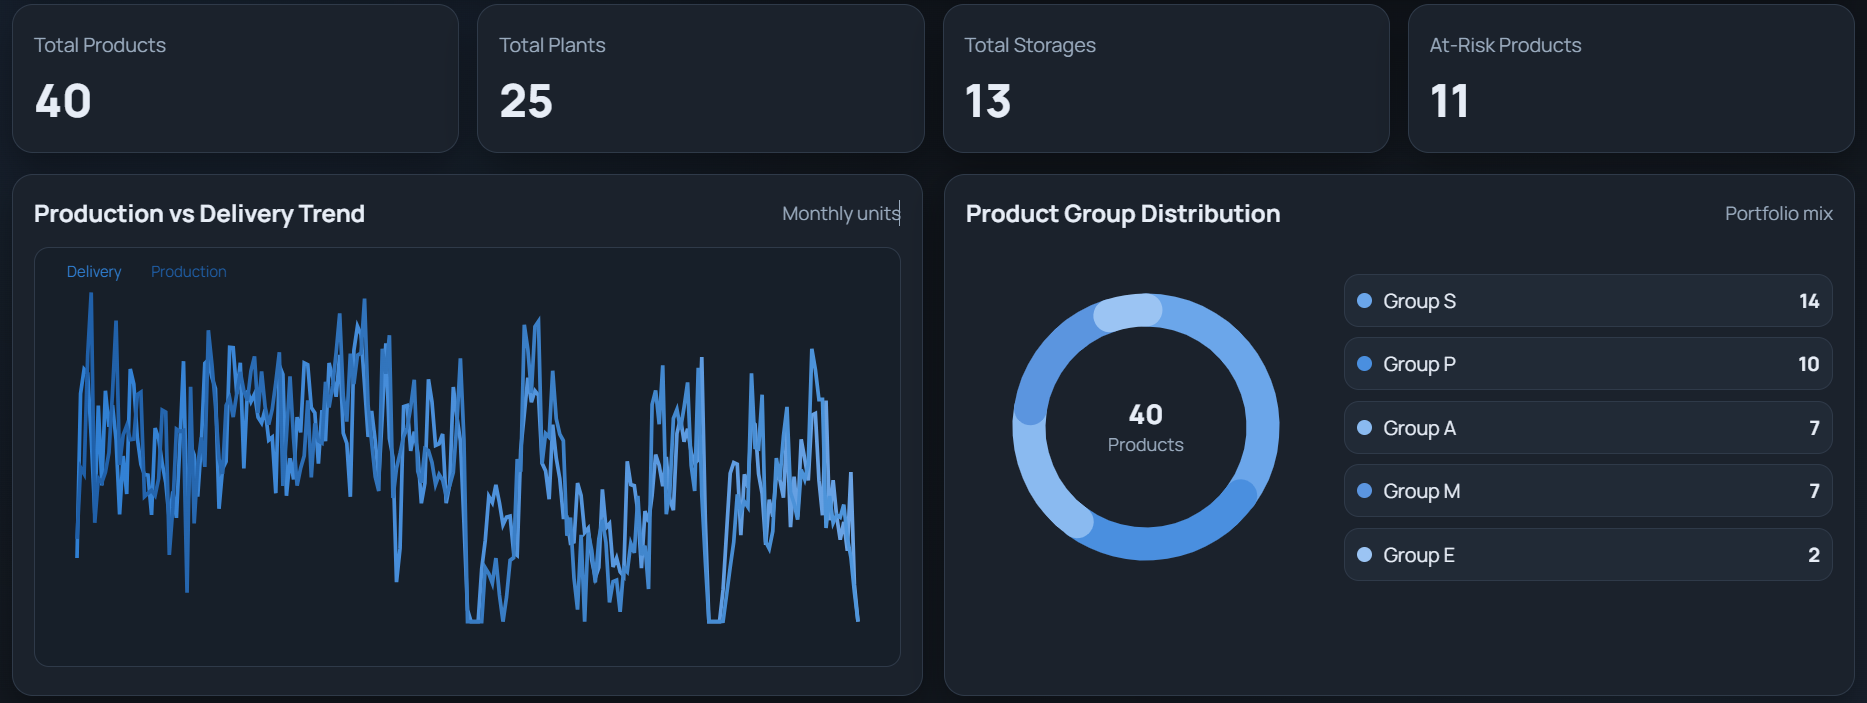
\includegraphics[width=0.95\linewidth]{figures/dashboard_overview.png}
\caption{EventualSmartFactory Overview panel displaying KPI cards, production vs delivery area chart, group distribution donut, and risk profile summary.}
\label{fig:overview}
\end{figure}

\subsection{Dashboard Panels}

The \textbf{Overview} panel presents KPI cards for total delivery, production, and sales orders, alongside a production vs delivery area chart, a group distribution donut chart, top delivery bars, and a risk profile chart. This gives operations managers an immediate posture assessment of the supply chain.

The \textbf{Factory Floor} panel provides plant load maps with fulfillment ratios, storage pressure bars, a risk watchlist table ranking products by fulfillment weakness, and a product inspector with filtering and drill-down capabilities. This panel supports the diagnostic phase of the operational workflow.

\begin{figure}[H]
    \centering

    \begin{minipage}{0.49\linewidth}
        \centering
        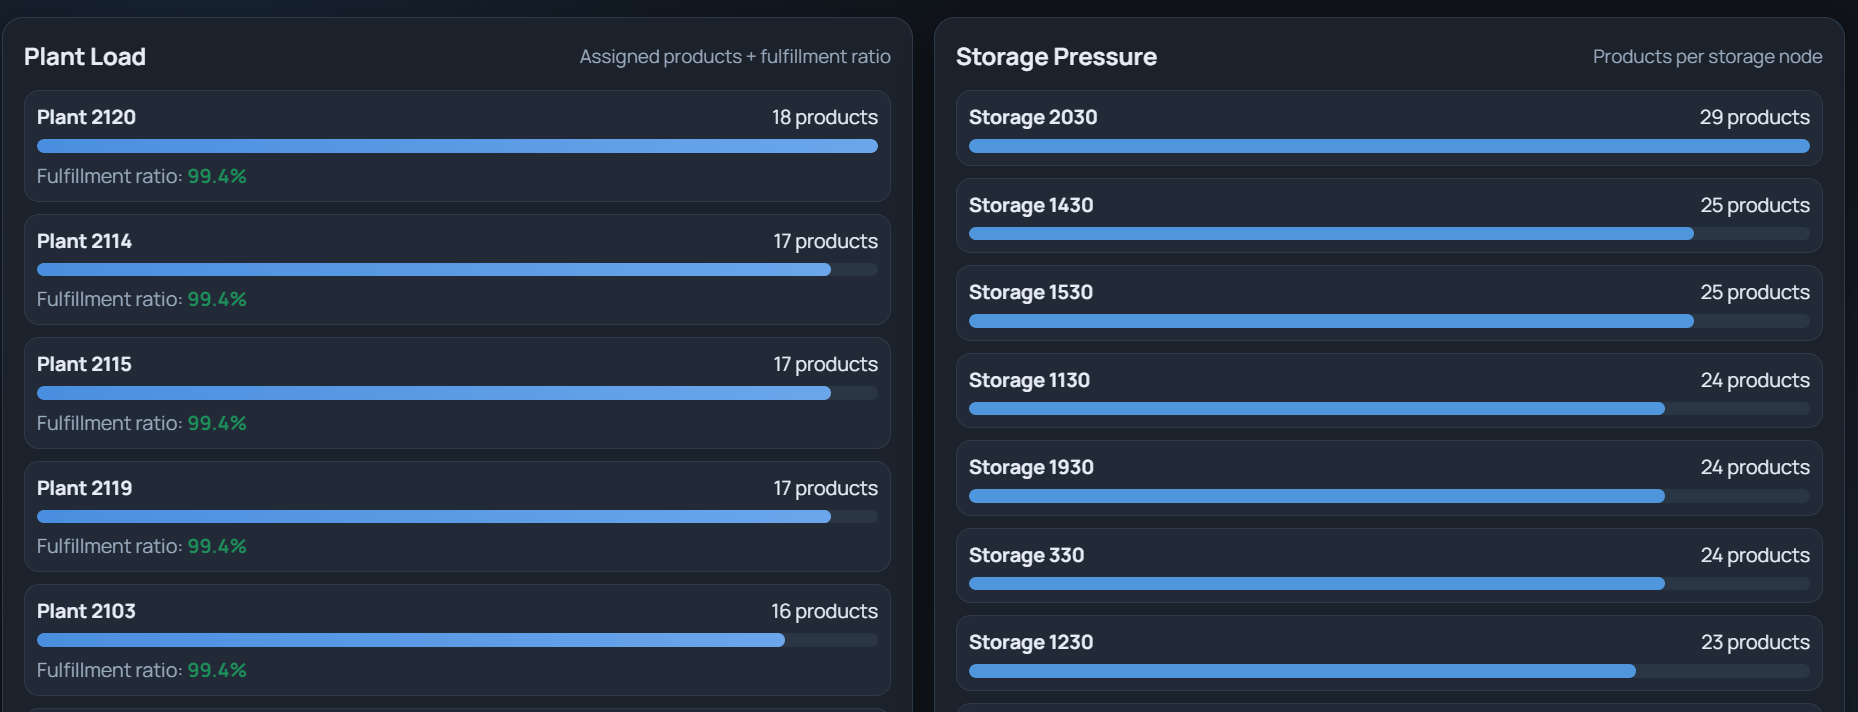
\includegraphics[width=\linewidth]{figures/factory_floor1.png}
    \end{minipage}
    \hfill
    \begin{minipage}{0.49\linewidth}
        \centering
        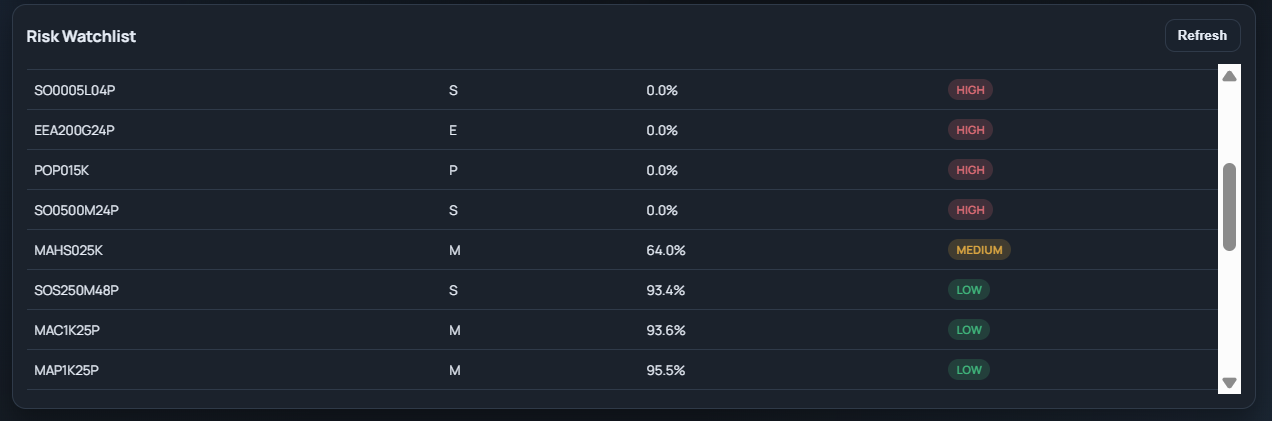
\includegraphics[width=\linewidth]{figures/factory_floor2.png}
    \end{minipage}

    \caption{Factory Floor panels showing plant load with fulfillment ratios, storage pressure bars, and the risk watchlist table ranking products by fulfillment weakness.}
    \label{fig:factory}
\end{figure}

The \textbf{AI Copilot} panel offers a conversational interface where users ask natural language questions about the supply chain. Each response displays the selected strategy, routing reason, and benchmark reference scores, providing full transparency into how the answer was generated. This traceability is critical for user trust in operational settings.

\begin{figure}[H]
\centering
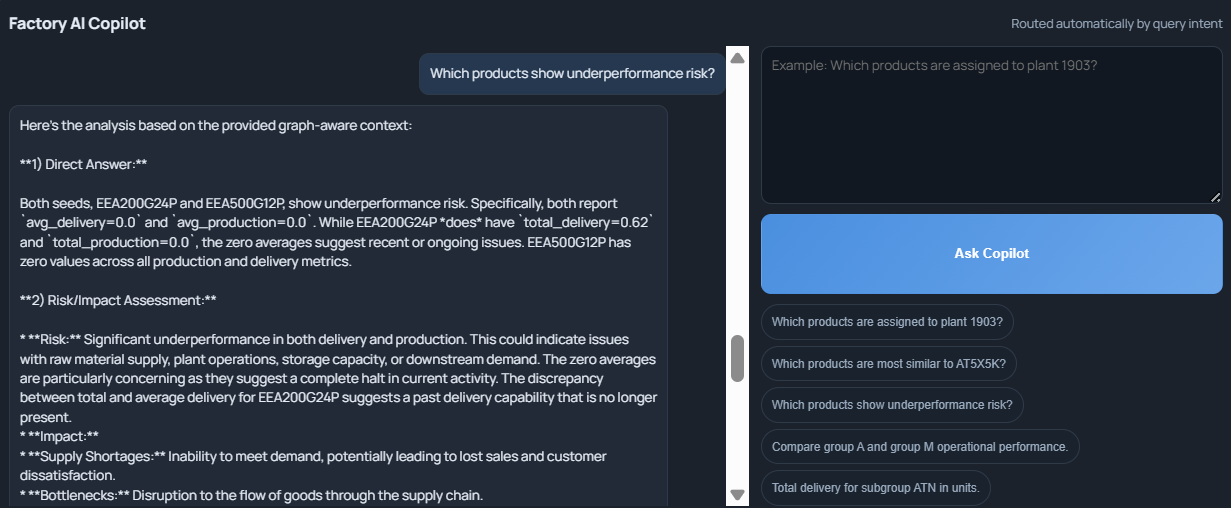
\includegraphics[width=0.8\linewidth]{figures/ai_copilot.png}
\caption{AI Copilot panel showing a natural language query and the generated answer.}
\label{fig:copilot}
\end{figure}

\subsection{User Journey}

The dashboard supports a practical corporate workflow that moves through five stages: \textit{monitor} (review KPIs and trend charts), \textit{diagnose} (check the risk watchlist for weak fulfillment products), \textit{investigate} (inspect plant and storage pressure in the Factory Floor panel), \textit{ask AI} (query the copilot with targeted questions), and \textit{decide} (take evidence-backed action). This creates a coherent loop from observation to decision, grounded in data at every step.

% ══════════════════════════════════════════════
\section{Business Implications}

\subsection{Operational Impact}

A routing-based RAG system offers several practical advantages for supply chain operations. The most immediate is \textbf{reduced triage time}. Operations teams currently spend significant time cross-referencing spreadsheets to diagnose delivery shortfalls. An AI copilot that can answer ``Why did product X under-deliver last week?'' with graph-grounded evidence could reduce triage from hours to minutes. The GraphRAG approach is particularly valuable here because it automatically surfaces related products through shared infrastructure-information that would require multiple manual lookups in a traditional workflow.

\textbf{Proactive risk identification} is another key benefit. The risk monitoring panel surfaces weak fulfillment ratios before they become critical. Combined with the copilot's reasoning capability, teams can investigate at-risk products and their upstream dependencies in a single workflow. In the 20-question DeepSeek-judge run, reasoning performance remained high (Gemini 4.40, GraphRAG 4.47), suggesting that even a mid-tier free generation model can provide useful risk signals when retrieval context is well-structured.

\textbf{Democratized data access} through Text2Cypher eliminates the need for analysts to write Cypher or SQL. Any team member can ask ``How many products are assigned to plant 1903?'' and receive an exact answer. This lowers the barrier to data-driven decision-making, particularly in organizations where database skills are concentrated in a small technical team. The deterministic routing ensures that structured queries are handled by the highest-precision path (5.00 structural average and 4.20 analytical average), rather than relying on approximate semantic retrieval.

Finally, unlike black-box prediction models, RAG systems provide \textbf{evidence-backed decisions} by citing the retrieved evidence that supports each answer. The routing metadata displayed in the copilot panel allows users to understand not only \textit{what} the system concluded but \textit{how} it arrived at that conclusion, which strategy was selected and why. This transparency is essential in operational contexts where decisions must be justified.

\subsection{Cost Savings: Industry Evidence}

The business case for AI-driven supply chain intelligence is supported by substantial industry evidence. According to McKinsey research, integrating AI in supply chain operations can reduce logistics costs by 5 to 20 percent. A February 2026 Accenture study (``Making Self-Funding Supply Chains Real'') found that AI could reduce operational expenditure by up to 24\% and cut manual interventions by as much as 50\% as autonomous systems scale up, lowering overall supply chain costs by up to 20\% depending on organizational maturity.

At the enterprise level, the impact is concrete. A Fortune 500 manufacturer with \pounds12~billion in revenue used AI-driven procurement optimization to identify \pounds24~million in savings by reclassifying spend data, revealing duplicate suppliers, and tightening price controls. A global asset manager used AI to optimize customer support operations and cut operating expenses by one-third, equivalent to approximately \pounds80~million. In warehousing, companies deploying AI-powered robotics and smart routing have reduced order fulfillment costs by 25\% in their most advanced facilities.

For a system like SupplyGraphOps, the most relevant impact area is \textbf{operational decision speed}. Industry data from StartUs Insights shows that early adopters of AI in supply chains improve logistics costs by 15\%, inventory levels by 35\%, and service levels by 65\%. The AI Index Report 2025 found that 43\% of businesses adopting AI in supply chain management register measurable cost savings, while 63\% see revenue gains. Studies on AI implementations for cost reduction report typical ROI between 150\% and 300\% within the first year.

To illustrate with a concrete scenario: consider a mid-sized supply chain operation spending \$2~million annually on logistics and operations. Based on the conservative end of McKinsey's 5-20\% range, AI-driven supply chain intelligence could save \$100{,}000 to \$400{,}000 per year. At the Accenture benchmark of 24\% OpEx reduction, the savings reach \$480{,}000. Even accounting for implementation costs (infrastructure, API fees at production scale, and integration effort), the payback period for AI supply chain tools typically falls between 12 and 18 months, with experienced companies reporting an average ROI of 4.3\%.

Between 2026 and 2030, AI-driven supply chains are projected to cut operational costs by \$1.3~trillion globally, as companies shift toward self-healing networks, real-time optimization, and AI-enhanced logistics ecosystems. Organizations that invest in AI-native supply chain infrastructure now will be positioned to capture a disproportionate share of these gains as the technology matures.

\subsection{Cost of the Experimental Prototype}

A notable aspect of this project is that the core pipeline-embedding generation, three RAG strategies, and interactive copilot-was built with low-cost/free-tier components using Gemma~3~27B and \texttt{gemini-embedding-001}. The updated evaluation phase introduced DeepSeek as an independent judge to reduce same-model bias, while infrastructure remained a local Neo4j instance in Docker.

For production deployment, costs would scale modestly. Embedding generation is a one-time cost per product, cached and reused across sessions. LLM inference is per-query, with the rate-limited 5-second sleep replaced by a paid tier for responsive user experience. The routing architecture itself reduces costs by directing simple queries to Text2Cypher (requiring only one LLM call for Cypher generation) rather than the embedding + retrieval + generation pipeline of RAG approaches. Based on current Google AI pricing, a production deployment serving 1{,}000 queries per day would cost approximately \$50-100/month-a fraction of the operational savings it enables.

\subsection{Limitations and Risks}

The original LLM-as-judge baseline used Gemma~3~27B as both generator and judge and showed leniency toward well-structured but incomplete answers. We mitigated this with a DeepSeek-judge rerun over 20 questions, but production deployment should still include human expert evaluation for high-stakes decisions. With 40 products, the current system remains a proof of concept; scaling to thousands of products would require re-evaluating embedding strategies and graph traversal performance. The seed-bias limitation in GraphRAG means that cross-group or global questions remain a weakness, addressable through multi-seed retrieval. Text2Cypher remains fragile on open-ended prompts, mitigated operationally by deterministic routing and GraphRAG fallback.

% ══════════════════════════════════════════════
\section{Lessons Learned}

The benchmark revealed clear specialization across retrieval strategies: Text2Cypher for exact analytical queries (4.20), GraphRAG for semantic and reasoning (4.33 and 4.47), and Semantic RAG for narrative breadth, arguing strongly against monolithic RAG pipelines. Node2Vec's failure reinforced a deeper point: embedding spaces are not interchangeable. The asymmetric retrieval problem, where query and document vectors come from fundamentally incompatible models, is a theoretical limitation, not a tuning issue. Routing should therefore be deterministic and keyword-based rather than LLM-delegated; it is faster, auditable, and gives operations teams transparency into why a strategy was selected.
\\ \\
Gemma 3 27B, deliberately chosen as a mid-tier free model, was sufficient to validate the architecture. The insight of which approach works best for which question type holds regardless of model quality; absolute scores would improve with a frontier model, but the specialization pattern would not change. This suggests a practical development strategy: validate architecture cheaply, then scale model quality for production. A final lesson is that honest partial answers outperform confident wrong ones. GraphRAG's acknowledgment that a subgraph does not contain a requested node is a better operational outcome than a hallucinated response, a property critical in high-stakes environments.
% ══════════════════════════════════════════════
\section*{References}

\begin{enumerate}[label={[\arabic*]}, nosep, leftmargin=*]
  \item Aziz, A., et al. ``SupplyGraph: A Benchmark Dataset for Graph-Based Supply Chain Analytics.'' \textit{CIOL Research Lab}, 2024.
  \item Lewis, P., et al. ``Retrieval-Augmented Generation for Knowledge-Intensive NLP Tasks.'' \textit{NeurIPS}, 2020.
  \item Edge, D., et al. ``From Local to Global: A Graph RAG Approach to Query-Focused Summarization.'' \textit{Microsoft Research}, arXiv:2404.16130, 2024.
  \item Microsoft Research. ``GraphRAG: Improving Global Search via Dynamic Community Selection.'' \textit{Microsoft Research Blog}, November 2024.
  \item Grover, A. and Leskovec, J. ``node2vec: Scalable Feature Learning for Networks.'' \textit{KDD}, 2016.
  \item Google DeepMind. ``Gemma 3 Technical Report.'' 2025.
  \item Google. ``Gemini Embedding API Documentation.'' 2025.
  \item McKinsey \& Company. ``AI-Driven Supply Chain Operations: Cost Reduction Benchmarks.'' 2025.
  \item Accenture. ``Making Self-Funding Supply Chains Real.'' February 2026.
  \item StartUs Insights. ``AI in Supply Chain: A Strategic Guide 2025-2030.'' 2025.
  \item Stanford University. ``AI Index Report 2025.'' 2025.
\end{enumerate}

\vspace{12pt}

% ══════════════════════════════════════════════
\section*{Appendix: System Architecture Diagram}

\begin{figure}[H]
\centering
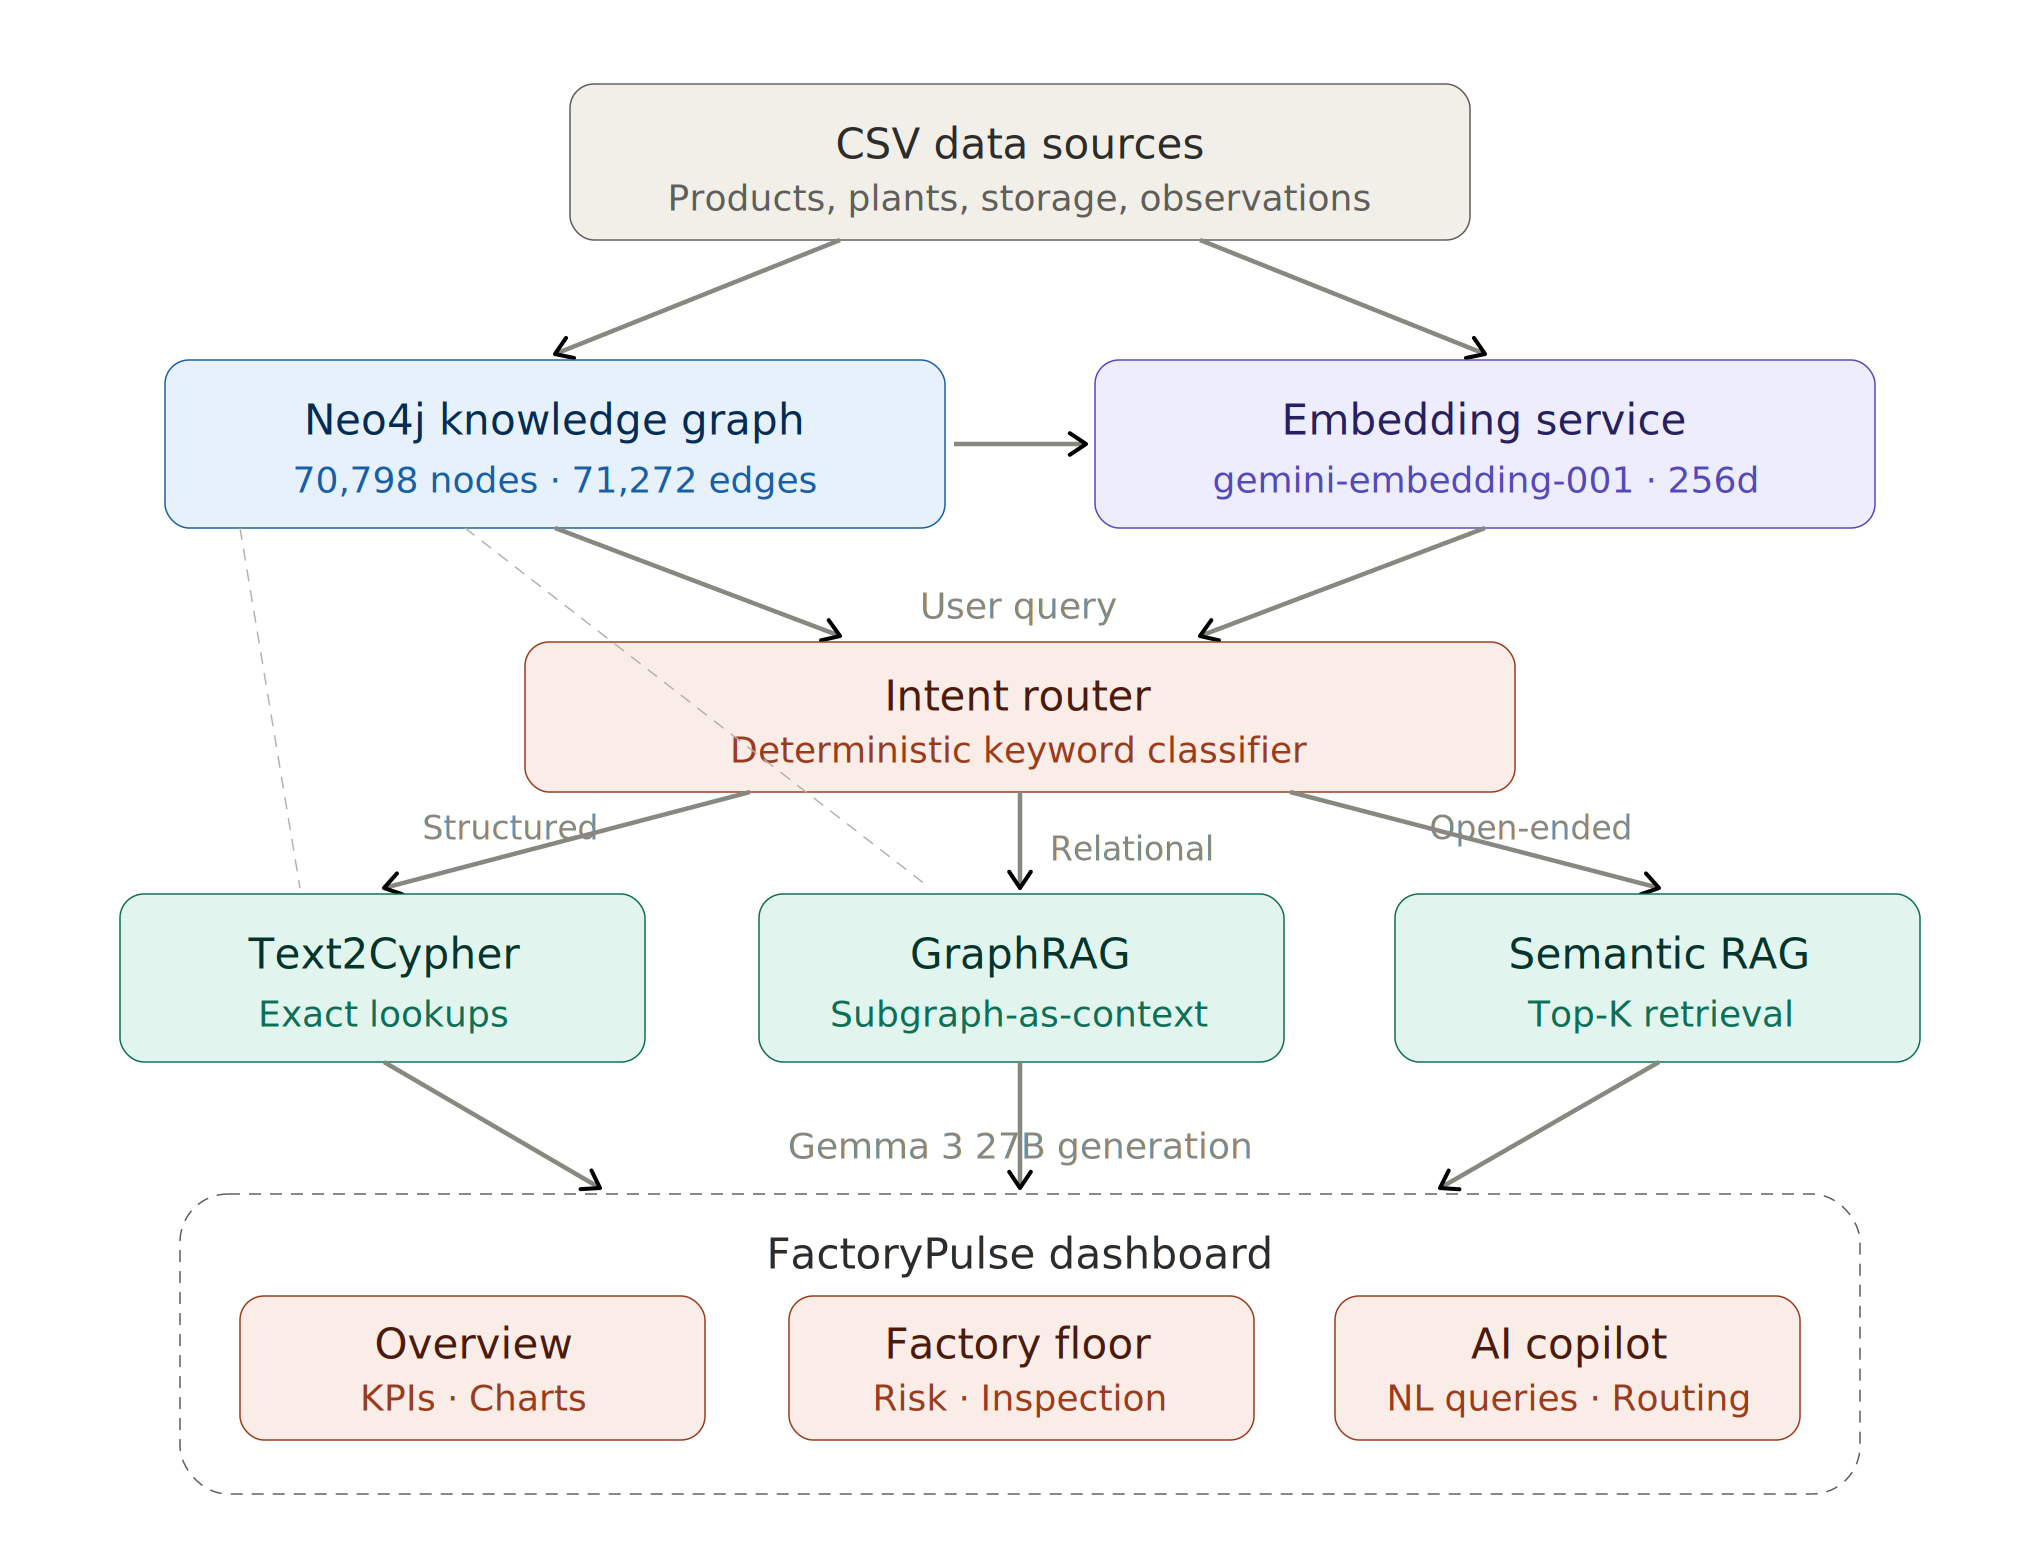
\includegraphics[width=0.95\linewidth]{figures/architecture.png}
\caption{SupplyGraphOps system architecture. CSV data is ingested into Neo4j and the embedding service. The intent router classifies user queries and dispatches them to the optimal retrieval strategy. Results are generated by Gemma~3~27B and displayed in the EventualSmartFactory dashboard.}
\label{fig:architecture}
\end{figure}

\end{document}
